% =============================================================================
%  Rapport d'ingénierie des données — Projet 3 : modern data stack e-commerce (FR)
%  Compilation : latexmk -xelatex rapport-fr.tex
% =============================================================================
\documentclass[11pt, a4paper, oneside, headings=normal, numbers=noenddot, DIV=12]{scrartcl}
\usepackage[french]{babel}
\usepackage{report-style}
\graphicspath{{../livraison/figures/fr/}}
\sisetup{locale=FR, group-minimum-digits=4}

% --- Métadonnées ---------------------------------------------------------------
\newcommand{\ReportAuthor}{LUMU BAMANA MANASSE}
\newcommand{\ReportAuthorRole}{Data engineer}
\newcommand{\ReportShortTitle}{E-commerce brésilien · Rapport d'ingénierie des données}
\newcommand{\ReportFooter}{Octobre 2026 · v1.0.0}
\newcommand{\ReportKicker}{Rapport d'ingénierie des données · Projet 3}
\newcommand{\ReportTitle}{Faut-il vendre\\au Brésil ?}
\newcommand{\ReportSubtitle}{Une modern data stack locale sur 100\,000 commandes réelles :\\data lake S3, dbt, DuckDB, Dagster, Docker et intégration continue}
\newcommand{\ReportMeta}{%
  \begin{tabularx}{\linewidth}{@{}>{\bfseries}l@{\hspace{1em}}Y@{}}
  Date & Octobre 2026 \\
  Version & 1.0.0 (livrée et recettée) \\
  Client & Maison Caju (entreprise fictive) · Mission CAJ-2026-001 \\
  Dépôt GitHub & \url{https://github.com/MediJr/olist-ecommerce-modern-data-stack} \\
  Langue & Français · \textit{English version available in the repository}
  \end{tabularx}}
\newcommand{\ReportScenario}{Scénario fictif, données réelles : l'entreprise cliente et ses interlocuteurs sont inventés pour simuler une mission
  professionnelle complète. Les données sont celles du \emph{Brazilian E-Commerce Public Dataset by Olist}, publié sur Kaggle sous licence
  CC BY-NC-SA 4.0 (commandes anonymisées de 2016 à 2018). Ce projet n'est ni commandé, ni validé, ni affilié à Olist.}
\hypersetup{pdftitle={Faut-il vendre au Brésil ? Rapport d'ingénierie des données}, pdfauthor={Lumu Bamana Manasse},
  pdfsubject={Modern data stack locale : S3, dbt, DuckDB, Dagster, projet de portfolio}, pdflang={fr-FR}}

\begin{document}
\sloppy
\MakeTitlePage

% =============================================================================
\section*{Fiche du document}
\addcontentsline{toc}{section}{Fiche du document}

\begin{tabularx}{\linewidth}{@{}>{\bfseries\sffamily}L{4.2cm}Y@{}}
\toprule
Projet & Projet 3 du portfolio : modern data stack (data lake, dbt, orchestration, CI) \\
Mission & CAJ-2026-001 : « Faut-il se lancer sur les marketplaces brésiliennes ? » \\
Client & Maison Caju, marque française de linge de maison (fictive), à l'attention de Claire Dumont \\
Auteur & Lumu Bamana Manasse, data engineer \\
Période de réalisation & Octobre 2026 \\
Données & Olist, 99\,441 commandes passées de septembre 2016 à octobre 2018 \\
Statut & \pill{good}{LIVRÉ} \pill{good}{RECETTÉ} \\
Code source & \url{https://github.com/MediJr/olist-ecommerce-modern-data-stack} \\
\bottomrule
\end{tabularx}

\subsection*{Historique des versions}
\begin{tabularx}{\linewidth}{@{}l l Y@{}}
\toprule
\textbf{Version} & \textbf{Date} & \textbf{Objet} \\
\midrule
0.1 & 23/10/2026 & Cadrage : brief, compte rendu, cahier des charges \\
0.5 & 23/10/2026 & Lac S3, ingestion, projet dbt, orchestration Dagster \\
0.9 & 25/10/2026 & Passage de toute la plateforme dans Docker, intégration continue, tableau de bord \\
1.0.0 & 25/10/2026 & Recette sur poste neuf, rapport final (français et anglais) \\
\bottomrule
\end{tabularx}

\subsection*{Guide de lecture}
\begin{tabularx}{\linewidth}{@{}>{\bfseries}L{4.2cm}Y@{}}
Comité de direction & \hyperref[sec:resume]{1. Résumé exécutif} et \hyperref[sec:resultats]{11. Résultats et recommandations} \\
Analyste (Hugo) & 6. Modèle de données dbt, 7. Qualité et tests, 9. Exploitation \\
Ingénieur reprenant le projet & 4. Architecture, 5. Pipeline et orchestration, 13. Retour d'expérience, annexes \\
\end{tabularx}

\begingroup
\addtokomafont{sectionentry}{\color{primary}}
\setcounter{tocdepth}{2}
\tableofcontents
\endgroup
\clearpage

% =============================================================================
\section{Résumé exécutif}\label{sec:resume}

\textbf{Le besoin.} Maison Caju envisage de vendre ses collections au Brésil via les marketplaces locales. Son comité de direction veut
une étude de marché chiffrée, et son analyste doit pouvoir \textbf{faire évoluer les indicateurs seul, en SQL, sans risque de régression}.
Les données arrivent par \textbf{livraisons mensuelles}.

\textbf{La solution.} Une \textbf{modern data stack} complète qui tient sur un poste et démarre avec une seule commande, \texttt{docker compose up} :
chaque livraison est contrôlée puis rangée dans un \textbf{data lake S3} (Parquet, une partition par mois). Elle est ensuite transformée par
\textbf{dbt} sur \textbf{DuckDB} en un schéma en étoile testé, orchestrée par \textbf{Dagster} (capteurs, partitions, rejeux), et servie
à un tableau de bord bilingue. Une \textbf{intégration continue} reconstruit et teste toute la chaîne à chaque modification.

\kpirow{99\,441}{commandes réelles\\(2016-2018)}{27 / 27}{exécutions réussies\\sur poste neuf}{18 min}{de zéro au\\tableau de bord}{94 / 94}{modèles et\\tests dbt}
\kpirow{0}{doublon\\au rejeu}{= source}{CA rapproché\\au centime}{14}{tests\\Python}{6}{décisions\\documentées (ADR)}

\begin{keybox}[Principaux résultats pour Maison Caju]
\begin{itemize}[leftmargin=1.2em]
  \item \textbf{Q1 · Où vendre :} 13,5~M BRL de chiffre d'affaires. L'univers maison pèse \textbf{19,8~\%}, et le linge de maison
        (\emph{bed\_bath\_table}) est la 3\textsuperscript{e} catégorie. São Paulo, Rio et Minas Gerais font \textbf{63~\%} du CA.
  \item \textbf{Q2 · Fidélité :} seuls \textbf{3,0~\%} des clients commandent deux fois. Ce marché se gagne par l'acquisition.
  \item \textbf{Q3 · Livraison :} la note passe de \textbf{4,3 à 2,1} dès 4 jours de retard. Le choix du transporteur est stratégique.
  \item \textbf{Q4 · Paiement :} carte bancaire à 75,5~\%, \emph{boleto} à 19,9~\%. Le panier triple avec le paiement en 7 à 10 fois.
  \item \textbf{Q5 · Fret :} 13,8~\% du prix à São Paulo, jusqu'à \textbf{28,5~\%} dans le Nord.
\end{itemize}
\end{keybox}

\textbf{Ce que démontre ce projet, côté ingénierie :} data lake S3 et format Parquet partitionné, contrat de livraison, ingestion idempotente,
modélisation dbt en couches avec tests de données, tests unitaires, contrat et rapprochements avec la source, orchestration par
événements avec Dagster, gestion de la concurrence d'un entrepôt à écrivain unique, conteneurisation complète et intégration continue.

% =============================================================================
\section{Contexte et cadrage}

\subsection{Ce que la demande implique techniquement}
\begin{table}[H]
\centering\small
\begin{tabularx}{\linewidth}{@{}L{5.4cm} Y@{}}
\toprule
\textbf{Demande du client} & \textbf{Conséquence technique} \\
\midrule
« Hugo doit faire évoluer les indicateurs sans casser ce qui marche » & Logique métier en \textbf{SQL versionné et testé} (dbt), \textbf{intégration continue} obligatoire \\
« Un jeu de données très détaillé » (9 tables) & \textbf{Modèle dimensionnel} : grain explicite, schéma en étoile \\
« Un tableau de bord pour le comité » & Il lit des tables \textbf{déjà calculées et testées}, jamais les fichiers bruts \\
Exports mensuels du partenaire & \textbf{Partitions} par livraison, \textbf{rejeu} sans doublon, \textbf{orchestrateur} \\
\bottomrule
\end{tabularx}
\caption{De la demande aux exigences techniques}
\end{table}

\subsection{Décisions du cadrage}
\begin{table}[H]
\centering\small
\begin{tabularx}{\linewidth}{@{}l L{3cm} Y@{}}
\toprule
\textbf{\#} & \textbf{Sujet} & \textbf{Décision} \\
\midrule
D1 & Mises à jour & Un export par mois ; simulé en découpant le jeu public par mois d'achat \\
D2 & Chiffre d'affaires & Prix des articles, hors fret, commandes ni annulées ni indisponibles. Défini \textbf{une seule fois}, dans dbt \\
D3 & Client fidèle & Client identifié par \texttt{customer\_unique\_id} ; fidèle = au moins deux commandes valides \\
D4 & Tableau de bord & Metabase, remplacé ensuite par Streamlit (ADR 004) \\
D5 & Maintenance & Toute modification passe par une \emph{pull request} testée par l'intégration continue \\
D6 & Langue & Tables et colonnes en anglais ; documentation en français, rapport aussi en anglais \\
\bottomrule
\end{tabularx}
\caption{Décisions de la réunion de cadrage du 23/10/2026}
\end{table}

\subsection{Questions business}
\begin{table}[H]
\centering\small
\begin{tabularx}{\linewidth}{@{}l Y L{4.4cm}@{}}
\toprule
\textbf{\#} & \textbf{Question} & \textbf{Décision éclairée} \\
\midrule
Q1 & Quelles catégories et quels États font le CA, et comment évolue-t-il ? & Collections et régions de lancement \\
Q2 & Quelle part des clients revient acheter ? & Fidélisation ou acquisition \\
Q3 & Le retard de livraison dégrade-t-il la note ? & Choix du transporteur \\
Q4 & Comment les clients paient-ils ? & Offre de paiement \\
Q5 & Combien pèse le fret selon l'État ? & Coût logistique par région \\
\bottomrule
\end{tabularx}
\caption{Les cinq questions retenues}
\end{table}

% =============================================================================
\section{Sources et profilage}

\subsection{Le jeu de données}
Le \emph{Brazilian E-Commerce Public Dataset by Olist} décrit environ \num{100000} commandes anonymisées passées sur une marketplace
brésilienne entre 2016 et 2018. Il compte \textbf{9 fichiers CSV liés} : commandes, articles, paiements, avis, clients, vendeurs, produits,
géolocalisation et traduction des catégories. Le client l'a téléchargé sur Kaggle (compte personnel requis), puis déposé dans
\texttt{data/source/}.

\subsection{Ce que le profilage a révélé}
\begin{table}[H]
\centering\small
\begin{tabularx}{\linewidth}{@{}L{5.6cm} Y@{}}
\toprule
\textbf{Constat} & \textbf{Risque si on l'ignore, et traitement} \\
\midrule
\texttt{customer\_id} : \num{99441} valeurs pour \num{96096} personnes (\texttt{customer\_unique\_id}) & Il change à chaque commande : la fidélité paraîtrait \textbf{nulle}. Compter sur \texttt{customer\_unique\_id} \\
\num{2961} commandes réglées en plusieurs paiements (jusqu'à 29) ; \num{9803} commandes à plusieurs articles & Une jointure articles × paiements \textbf{multiplie le CA}. Agréger chaque table avant de joindre \\
\num{98410} \texttt{review\_id} pour \num{99224} avis & Le \texttt{review\_id} seul n'est pas une clé : clé composite (\texttt{review\_id}, \texttt{order\_id}) \\
2 catégories sans traduction, 610 produits sans catégorie & Cases vides dans le tableau de bord : repli explicite et testé (\texttt{unknown}) \\
775 commandes sans article ; 8 commandes « livrées » sans date de livraison & Exclues du CA ou des délais, de façon explicite \\
\num{1000163} points GPS pour \num{19015} préfixes de code postal, dont certains hors du Brésil & Médiane par préfixe, après filtrage géographique \\
Novembre 2016 : aucune commande ; septembre-octobre 2018 : 20 commandes, presque toutes annulées & Une livraison vide reste une livraison ; analyses sur les mois complets (01/2017-08/2018) \\
\bottomrule
\end{tabularx}
\caption{Profilage : sept pièges, sept traitements}
\end{table}

% =============================================================================
\section{Architecture}

\begin{figure}[H]
\centering
\resizebox{\linewidth}{!}{%
\begin{tikzpicture}[
  font=\sffamily\small, node distance=0.6cm and 0.75cm,
  src/.style={draw=rule, fill=panel, rounded corners=2pt, minimum width=2.4cm, minimum height=1.1cm, align=center},
  stage/.style={draw=primary, fill=primary, text=white, rounded corners=3pt, minimum width=2.2cm, minimum height=1.2cm, align=center, font=\sffamily\small\bfseries},
  store/.style={cylinder, shape border rotate=90, aspect=0.18, draw=accent, fill=accent!8, minimum width=2.3cm, minimum height=1.3cm, align=center},
  arr/.style={-{Stealth[length=2.6mm]}, thick, color=ink2}]
  \node[src] (p) {Partenaire\\\scriptsize CSV + \_SUCCESS};
  \node[stage, right=of p] (i) {INGESTION\\\scriptsize\mdseries contrat};
  \node[store, right=of i] (b) {\scriptsize Lac S3 · bronze\\\scriptsize Parquet / mois};
  \node[stage, right=of b] (s) {STAGING\\\scriptsize\mdseries typage};
  \node[stage, right=of s] (m) {INTERM.\\\scriptsize\mdseries règles};
  \node[store, right=of m] (w) {\scriptsize DuckDB · marts\\\scriptsize étoile};
  \node[src, right=of w] (d) {Streamlit\\\scriptsize FR / EN};
  \node[src, above=0.9cm of b, fill=white, draw=primary] (dag) {\textbf{Dagster}\\\scriptsize capteurs · partitions};
  \draw[arr] (p) -- (i); \draw[arr] (i) -- (b); \draw[arr] (b) -- (s); \draw[arr] (s) -- (m); \draw[arr] (m) -- (w); \draw[arr] (w) -- (d);
  \draw[arr, dashed] (dag) -| (i); \draw[arr, dashed] (dag) -| (m);
  \begin{scope}[on background layer]
    \node[draw=rule, dashed, rounded corners=6pt, fit=(s)(m)(w), inner sep=8pt, label={[font=\scriptsize\sffamily, text=ink2]below:dbt build (modèles + tests)}] {};
  \end{scope}
\end{tikzpicture}}
\caption{De la livraison au tableau de bord}
\end{figure}

\begin{table}[H]
\centering\small
\begin{tabularx}{\linewidth}{@{}L{2.6cm} L{3.6cm} Y@{}}
\toprule
\textbf{Rôle} & \textbf{Choix} & \textbf{Pourquoi} \\
\midrule
Data lake & Stockage compatible S3 (SeaweedFS), Parquet & Même interface qu'Amazon S3 ou Google Cloud Storage : seul l'emplacement change pour passer au cloud \\
Entrepôt & DuckDB & Colonnaire, lit le Parquet sur S3 directement, rien à administrer \\
Transformations & dbt 1.12 & SQL versionné, testé, documenté, avec le lignage : maintenable par un analyste \\
Orchestration & Dagster 1.13 & Raisonne en \emph{assets} ; chaque modèle dbt devient un asset et chaque test un contrôle \\
Restitution & Streamlit & Tableau de bord versionné et testé, lecture seule sur l'entrepôt \\
Exécution & Docker Compose & Trois services ; image unique \texttt{python:3.13-slim}, versions figées \\
Qualité & GitHub Actions & Toute la chaîne reconstruite et testée à chaque \emph{pull request} \\
\bottomrule
\end{tabularx}
\caption{Choix techniques (ADR 001, 002, 004, 005)}
\end{table}

Le lac est désigné par une seule variable, \texttt{LAKE\_URI} : \texttt{s3://olist-lake} en exploitation, un simple dossier dans
l'intégration continue. \textbf{Le code ne fait pas la différence} : c'est ce qui le rend transposable sur le cloud.

% =============================================================================
\section{Pipeline et orchestration}

\subsection{Le contrat de livraison}
Le partenaire dépose un dossier par mois. Il écrit le fichier \texttt{\_SUCCESS} \textbf{en dernier} : un dossier sans ce marqueur est
une livraison en cours, jamais lue. Avant toute écriture dans le lac, chaque fichier doit respecter son contrat :

\begin{itemize}[leftmargin=1.2em]
  \item un \textbf{en-tête identique} à celui attendu : une colonne ajoutée, renommée ou déplacée bloque l'ingestion (dérive de schéma) ;
  \item des \textbf{clés non vides et uniques} ;
  \item une lecture \textbf{tout en texte}, avec des colonnes déclarées : un mois vide (en-tête seul) se lit comme un mois plein.
\end{itemize}

\subsection{La couche bronze : idempotente par construction}
Chaque table d'un mois devient \textbf{un seul fichier Parquet}, rangé selon la convention Hive, que DuckDB, Spark et BigQuery lisent tous :

\begin{lstlisting}[language={}]
s3://olist-lake/bronze/orders/delivery_month=2017-01/orders.parquet
\end{lstlisting}

Rejouer un mois \textbf{remplace} ce fichier : un doublon est impossible. Deux colonnes de traçabilité sont ajoutées :
\texttt{\_source\_file} (fichier d'origine) et \texttt{\_ingested\_at} (heure d'entrée dans le lac).

\subsection{L'orchestration par événements}
\begin{table}[H]
\centering\small
\begin{tabularx}{\linewidth}{@{}L{3.6cm} Y@{}}
\toprule
\textbf{Mécanisme Dagster} & \textbf{Rôle} \\
\midrule
Partitions dynamiques & Une partition \texttt{delivery\_month} est créée à la \textbf{réception} d'une livraison, plutôt qu'un calendrier fixé à l'avance \\
Capteur \texttt{landing\_sensor} & Toutes les 30~s : une livraison nouvelle \textbf{ou relivrée} (marqueur modifié) déclenche le job \texttt{monthly\_delivery} \\
Clé d'exécution \texttt{mois@horodatage} & Une même version de livraison n'est jamais traitée deux fois \\
Limite de concurrence & DuckDB n'accepte qu'un écrivain : \textbf{une exécution à la fois} (\texttt{dagster.yaml}) \\
Amorçage & Le capteur mensuel attend les référentiels ; des référentiels arrivés seuls sont chargés sans dbt \\
Délai maximal & 15 minutes par exécution, surveillées par le démon : un blocage ne retient plus la file \\
\bottomrule
\end{tabularx}
\caption{Orchestration (ADR 006)}
\end{table}

% =============================================================================
\section{Modèle de données dbt}

\subsection{Trois couches, trois rôles}
\begin{table}[H]
\centering\small
\begin{tabularx}{\linewidth}{@{}L{2.6cm} L{2.2cm} Y@{}}
\toprule
\textbf{Couche} & \textbf{Modèles} & \textbf{Rôle} \\
\midrule
Staging (vues) & 9 & Un modèle par source : renommer, typer (\texttt{decimal} pour l'argent, jamais \texttt{float}), garder la dernière livraison. \textbf{Aucune règle métier} \\
Intermediate (vues) & 2 & \texttt{int\_orders} : une ligne par commande et \textbf{toutes} les règles métier, écrites une seule fois \\
Marts (tables) & 6 + 5 & Schéma en étoile, plus une table de reporting par question \\
\bottomrule
\end{tabularx}
\caption{Les 22 modèles dbt (ADR 003)}
\end{table}

\subsection{Le schéma en étoile}
La table de faits principale, \texttt{fct\_order\_items}, a pour \textbf{grain l'article vendu} : c'est le niveau le plus fin qui porte
le chiffre d'affaires. On peut toujours agréger vers le haut (commande, catégorie, mois), jamais redescendre. Elle est entourée de
\texttt{dim\_customers} (client réel), \texttt{dim\_products}, \texttt{dim\_sellers} et \texttt{dim\_date}. Une seconde table de faits,
\texttt{fct\_orders}, porte les mesures de la commande : livraison, avis, paiement.

\subsection{La règle qui évite de multiplier le chiffre d'affaires}
Une commande à 2 articles et 2 paiements produit \textbf{4 lignes} si l'on joint les tables brutes. \texttt{int\_orders} agrège donc chaque
table enfant \textbf{avant} la jointure :

\begin{lstlisting}[language=DuckSQL]
with items as (
    select order_id, count(*) as item_count, sum(price) as items_value,
           sum(freight_value) as freight_value
    from {{ ref('stg_order_items') }} group by order_id
),
payments as (
    select order_id, sum(payment_value) as payment_value, count(*) as payment_count
    from {{ ref('stg_order_payments') }} group by order_id
)
select ... from {{ ref('stg_orders') }} o
left join items using (order_id) left join payments using (order_id)
\end{lstlisting}

Cette règle est verrouillée par un \textbf{test unitaire dbt} (deux articles, deux paiements, montants attendus) et par un
\textbf{rapprochement} avec la source (section~\ref{sec:qualite}).

% =============================================================================
\section{Qualité et tests}\label{sec:qualite}

\begin{table}[H]
\centering\small
\begin{tabularx}{\linewidth}{@{}L{4.4cm} Y r@{}}
\toprule
\textbf{Type} & \textbf{Ce qui est vérifié} & \textbf{Nombre} \\
\midrule
Tests de données dbt & Unicité, non-nullité, relations, valeurs acceptées (statuts, notes, 27 États) & 69 \\
Tests unitaires dbt & Validité et retard ; non-multiplication des montants ; rang du client réel & 3 \\
Rapprochements (tests singuliers) & CA des marts = total bronze ; paiements = total bronze ; cohorte complète au mois 0 & 3 \\
Contrat imposé & Colonnes et types de \texttt{fct\_order\_items} & 1 \\
Tests Python (pytest) & Découpage des livraisons, contrat, idempotence, mois vide, tableau de bord & 14 \\
\bottomrule
\end{tabularx}
\caption{Les filets de sécurité}
\end{table}

\begin{keybox}[Le rapprochement avec la source]
Le test \texttt{assert\_revenue\_reconciles\_with\_source} recalcule le chiffre d'affaires \textbf{directement sur la couche bronze}, sans passer
par aucun modèle dbt, et le compare à celui du tableau de bord. Résultat : \textbf{\num{13494400.74}~BRL des deux côtés}, au centime près.
Si une jointure perd ou duplique un article, les deux totaux divergent et la construction échoue.
\end{keybox}

\subsection{Une intégration continue qui mord}
Pour la recette, une erreur classique a été introduite volontairement : \textbf{ajouter le fret au chiffre d'affaires}.

\begin{terminal}{dbt build · erreur volontaire}
\begin{lstlisting}[style=terminal]
# 1. fret ajouté : le type de la colonne change
Compilation Error in model fct_order_items
  This model has an enforced contract that failed.

# 2. fret ajouté, en gardant le même type
94 of 94 FAIL 1 assert_revenue_reconciles_with_source ......... [FAIL 1]
Done. PASS=93 WARN=0 ERROR=1 SKIP=0 TOTAL=94          (code de sortie : 1)
\end{lstlisting}
\end{terminal}

Les deux filets se complètent : le \textbf{contrat} protège la forme (colonnes, types), le \textbf{rapprochement} protège le fond (les montants).
Dans les deux cas, dbt sort en erreur : la \emph{pull request} serait refusée.

% =============================================================================
\section{Sécurité et données personnelles}
\begin{itemize}[leftmargin=1.2em]
  \item Données \textbf{anonymisées par l'éditeur} : identifiants hachés, ni nom ni adresse ; seuls la ville, l'État et le préfixe du code postal subsistent.
  \item Secrets (clés S3) dans \texttt{.env}, exclu de Git ; le fichier d'identités S3 est généré au démarrage du conteneur.
  \item Services exposés uniquement sur \texttt{127.0.0.1} ; conteneurs exécutés avec un \textbf{utilisateur sans privilèges}.
  \item Le tableau de bord monte l'entrepôt \textbf{en lecture seule}.
  \item Licence CC BY-NC-SA 4.0 : l'archive complète n'est pas redistribuée ; seul un échantillon de 450 commandes, attribué, sert à la CI.
\end{itemize}

% =============================================================================
\section{Exploitation}
\begin{table}[H]
\centering\small
\begin{tabularx}{\linewidth}{@{}L{4.6cm} Y@{}}
\toprule
\textbf{Besoin} & \textbf{Commande ou outil} \\
\midrule
Démarrer la plateforme & \texttt{docker compose up -d -{}-build} \\
Recevoir une livraison & Déposer le dossier du mois dans \texttt{data/landing/} : le capteur fait le reste \\
Rejouer un mois corrigé & Relivrer le dossier (nouveau \texttt{\_SUCCESS}) ou relancer la partition dans Dagster \\
Suivre les exécutions & Interface Dagster, \url{http://127.0.0.1:3000} : graphe, partitions, contrôles, journaux \\
Modifier un indicateur & Modifier le modèle dbt, puis \texttt{docker compose run -{}-rm dagster python -m olist\_pipeline.dbt\_cli build} \\
Lancer les tests Python & \texttt{docker compose run -{}-rm dagster pytest} \\
\bottomrule
\end{tabularx}
\caption{Gestes d'exploitation}
\end{table}

% =============================================================================
\section{Recette}
La recette a été passée sur un \textbf{poste neuf simulé} : volumes Docker supprimés, zone de dépôt vide. Les 26 livraisons et les
référentiels ont été déposés d'un coup, puis traités sans intervention : \textbf{27 exécutions réussies sur 27, en 18 minutes},
avec 19~s de traitement médian par mois.

\begin{table}[H]
\centering\small
\begin{tabularx}{\linewidth}{@{}l Y c@{}}
\toprule
\textbf{\#} & \textbf{Critère} & \textbf{Résultat} \\
\midrule
C1 & Lancement sur un poste neuf en suivant le README & \ok \\
C2 & Un mois = une partition ; traiter un mois ne retraite pas les autres & \ok \\
C3 & Rejouer un mois ne crée aucun doublon (octobre 2016 relivré : 329 commandes avant et après) & \ok \\
C4 & CA des marts égal au total de la source (\num{13494400.74}~BRL) & \ok \\
C5 & Tous les tests dbt passent (94/94) ; chaque modèle est documenté & \ok \\
C6 & L'intégration continue échoue si un test casse (démonstration ci-dessus) & \ok \\
C7 & Le tableau de bord répond à Q1-Q5 (5 onglets, 10 graphiques, FR/EN) & \ok \\
C8 & Aucun secret ni donnée brute versionné & \ok \\
\bottomrule
\end{tabularx}
\caption{Critères d'acceptation : 8 sur 8}
\end{table}

% =============================================================================
\section{Résultats et recommandations}\label{sec:resultats}

\subsection*{Q1 · Où se fait le chiffre d'affaires ?}
\begin{figure}[H]
\centering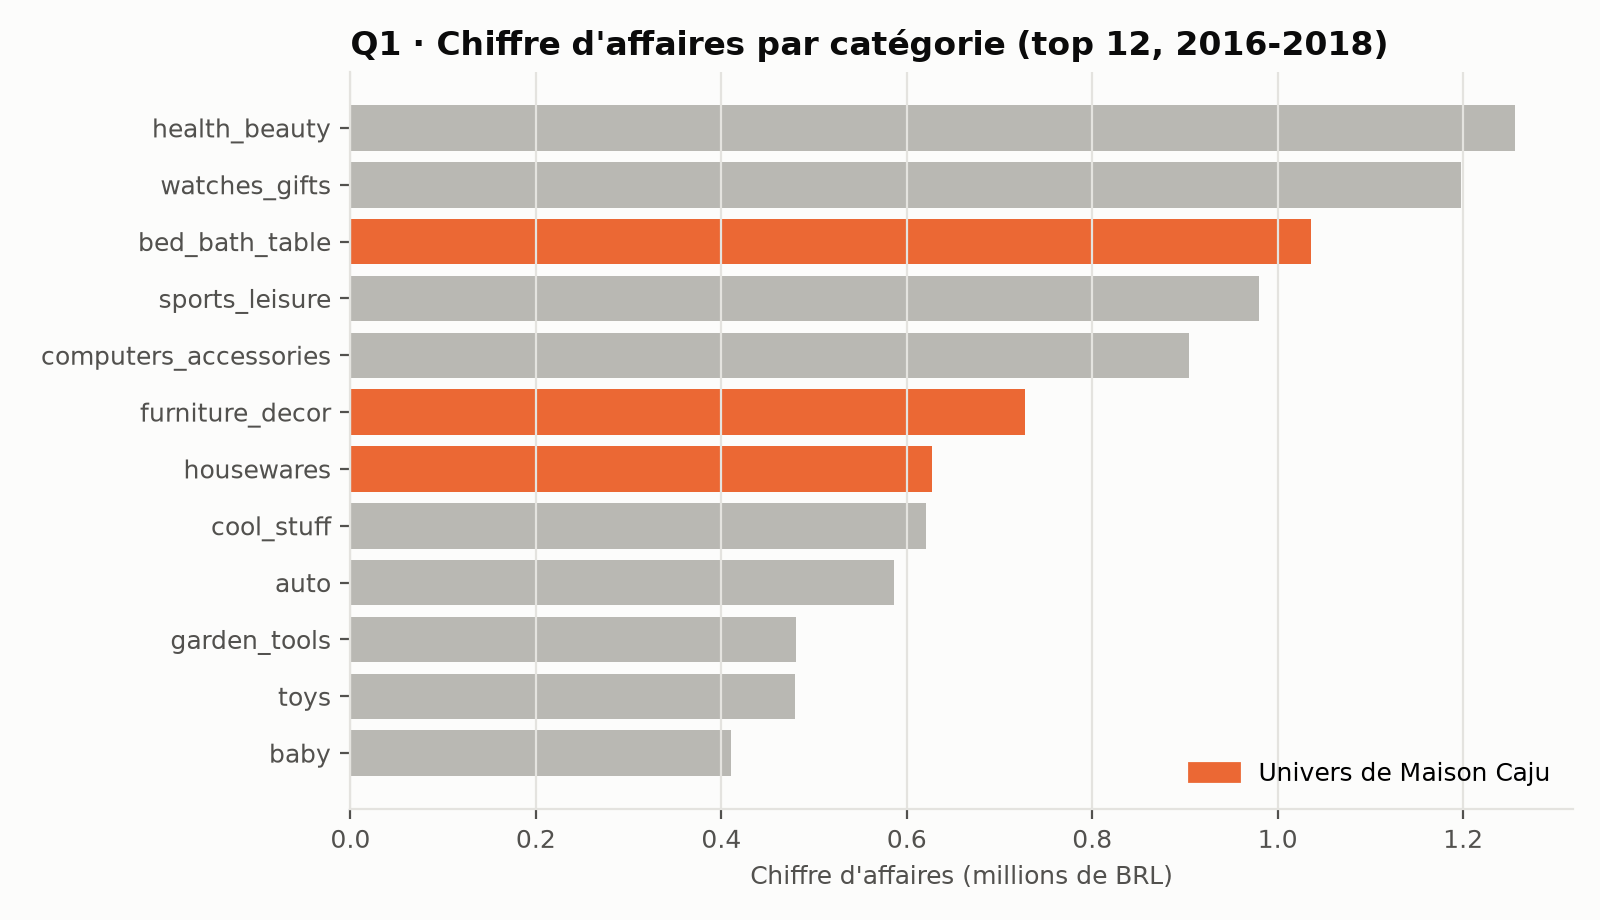
\includegraphics[width=0.86\linewidth]{q1_ca_par_categorie.png}
\end{figure}
Sur \num{98207} commandes valides, le chiffre d'affaires atteint \textbf{13,5~M BRL} (hors fret). L'univers de Maison Caju pèse
\textbf{19,8~\%}, et le linge de maison (\emph{bed\_bath\_table}, 7,7~\%) est la 3\textsuperscript{e} catégorie du marché.

\begin{figure}[H]
\centering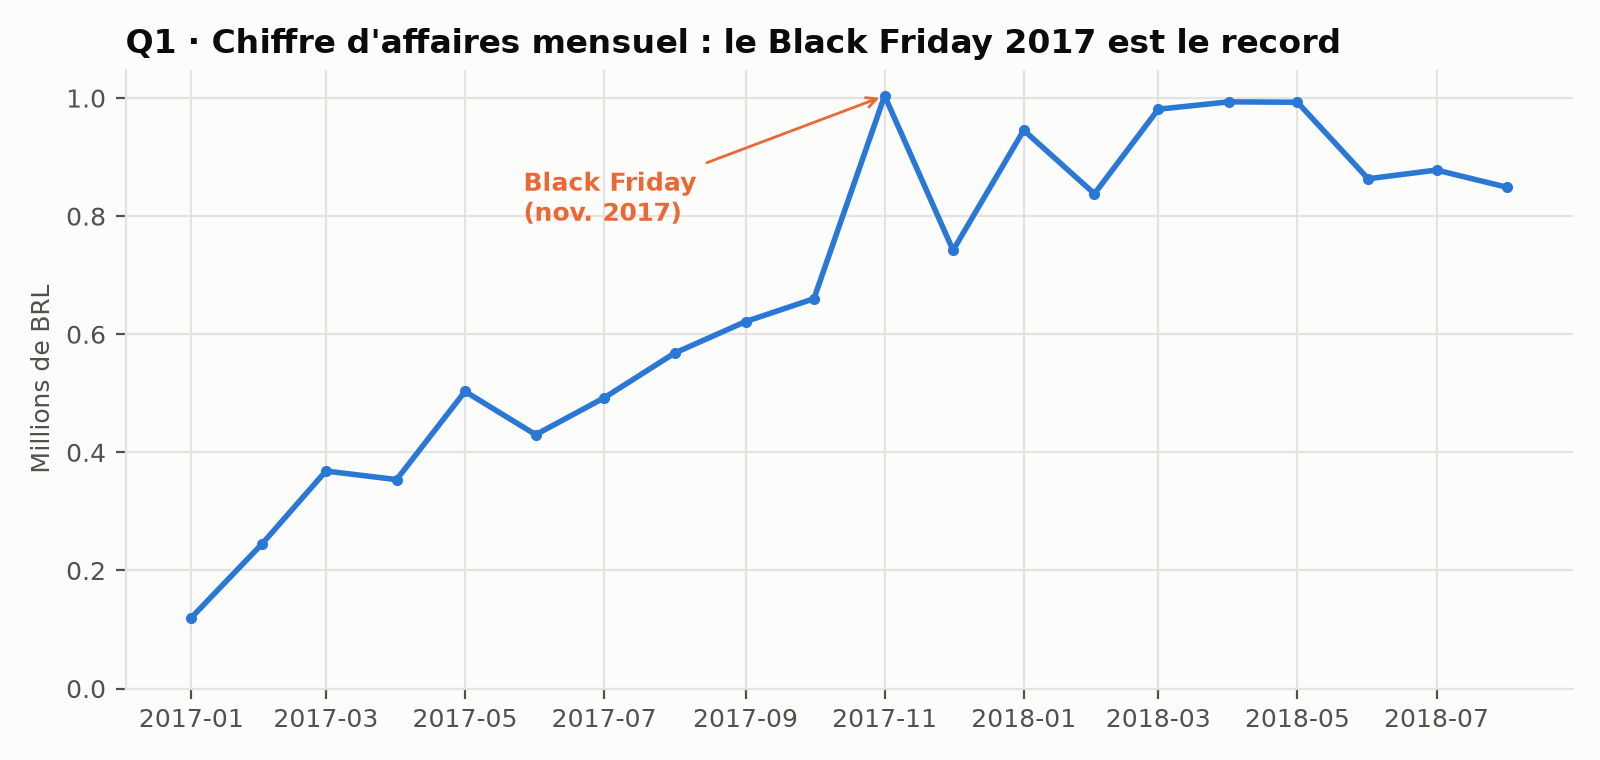
\includegraphics[width=0.86\linewidth]{q1b_ca_mensuel.png}
\end{figure}
Le marché croît fortement en 2017, puis se stabilise autour de 0,9~M BRL par mois en 2018. Le \textbf{Black Friday 2017} dépasse
octobre de \textbf{52~\%}.

\begin{figure}[H]
\centering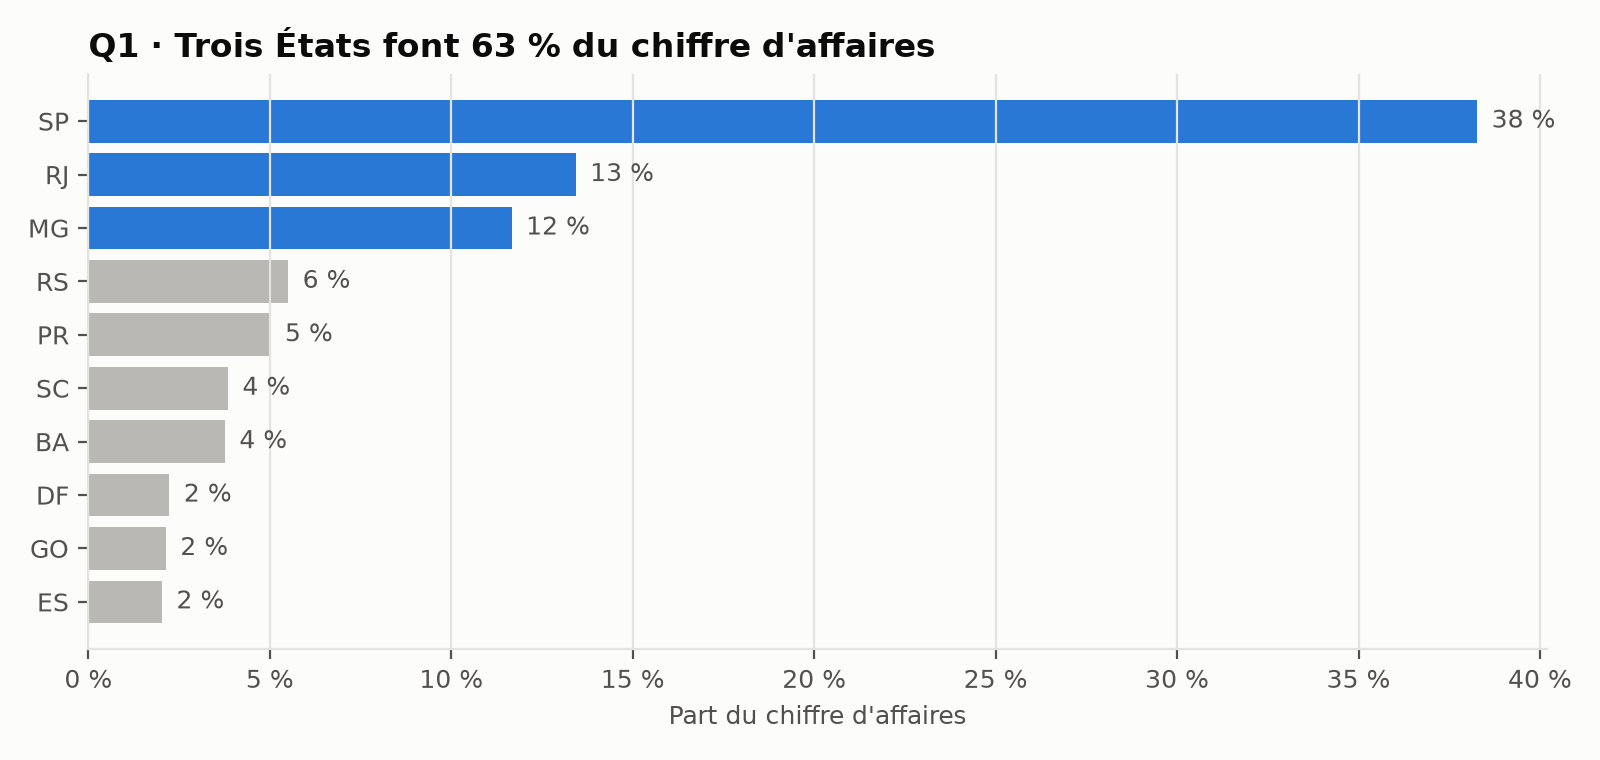
\includegraphics[width=0.86\linewidth]{q1c_ca_par_etat.png}
\end{figure}

\subsection*{Q2 · Les clients reviennent-ils ?}
\begin{figure}[H]
\centering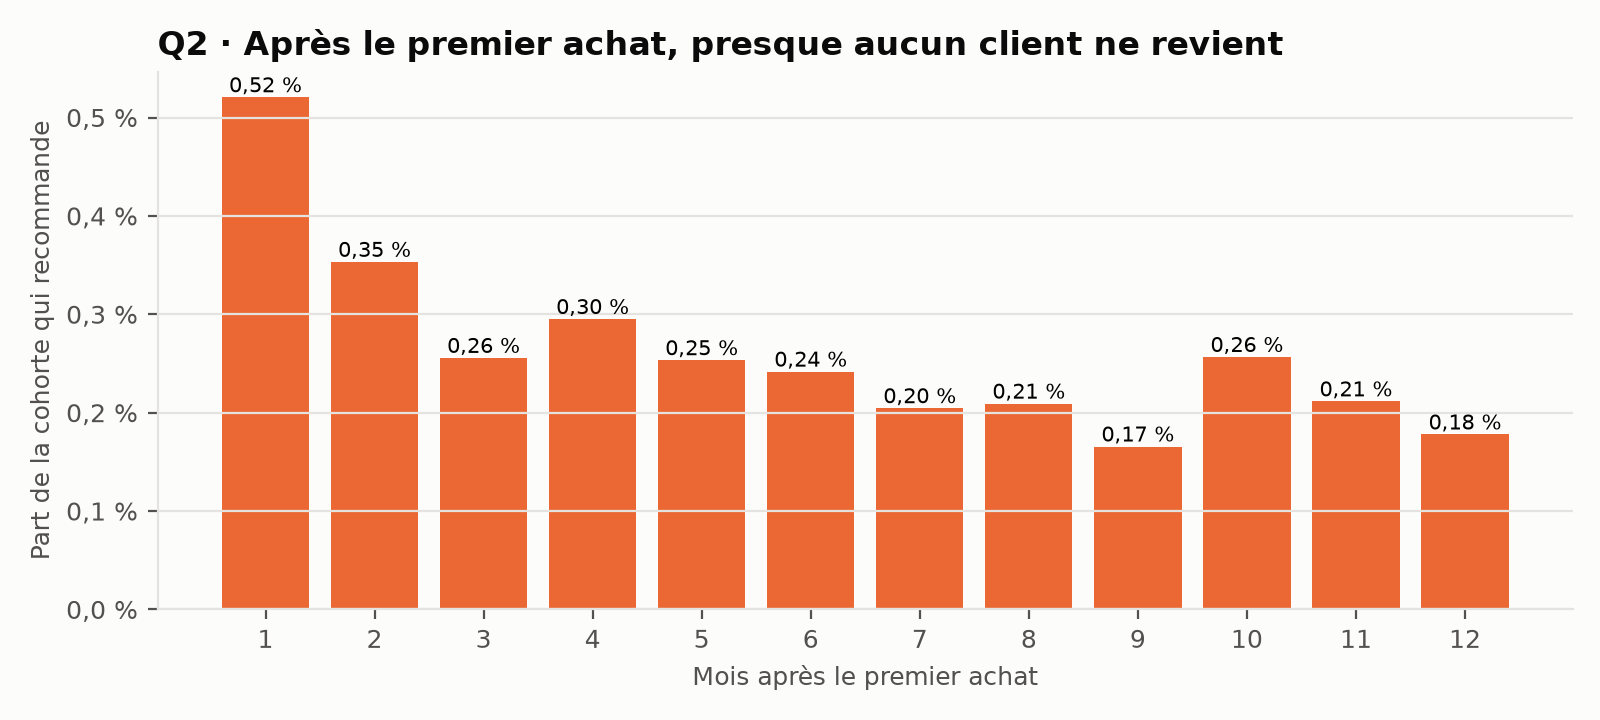
\includegraphics[width=0.86\linewidth]{q2_retention.png}
\end{figure}
Sur \num{94990} clients ayant passé une commande valide, seuls \textbf{\num{2888} (3,0~\%)} en ont passé une deuxième, 28 jours plus tard
en médiane. Un mois après leur premier achat, à peine \textbf{0,5~\%} des clients de 2017 recommandent.

\subsection*{Q3 · Le retard de livraison coûte-t-il des avis ?}
\begin{figure}[H]
\centering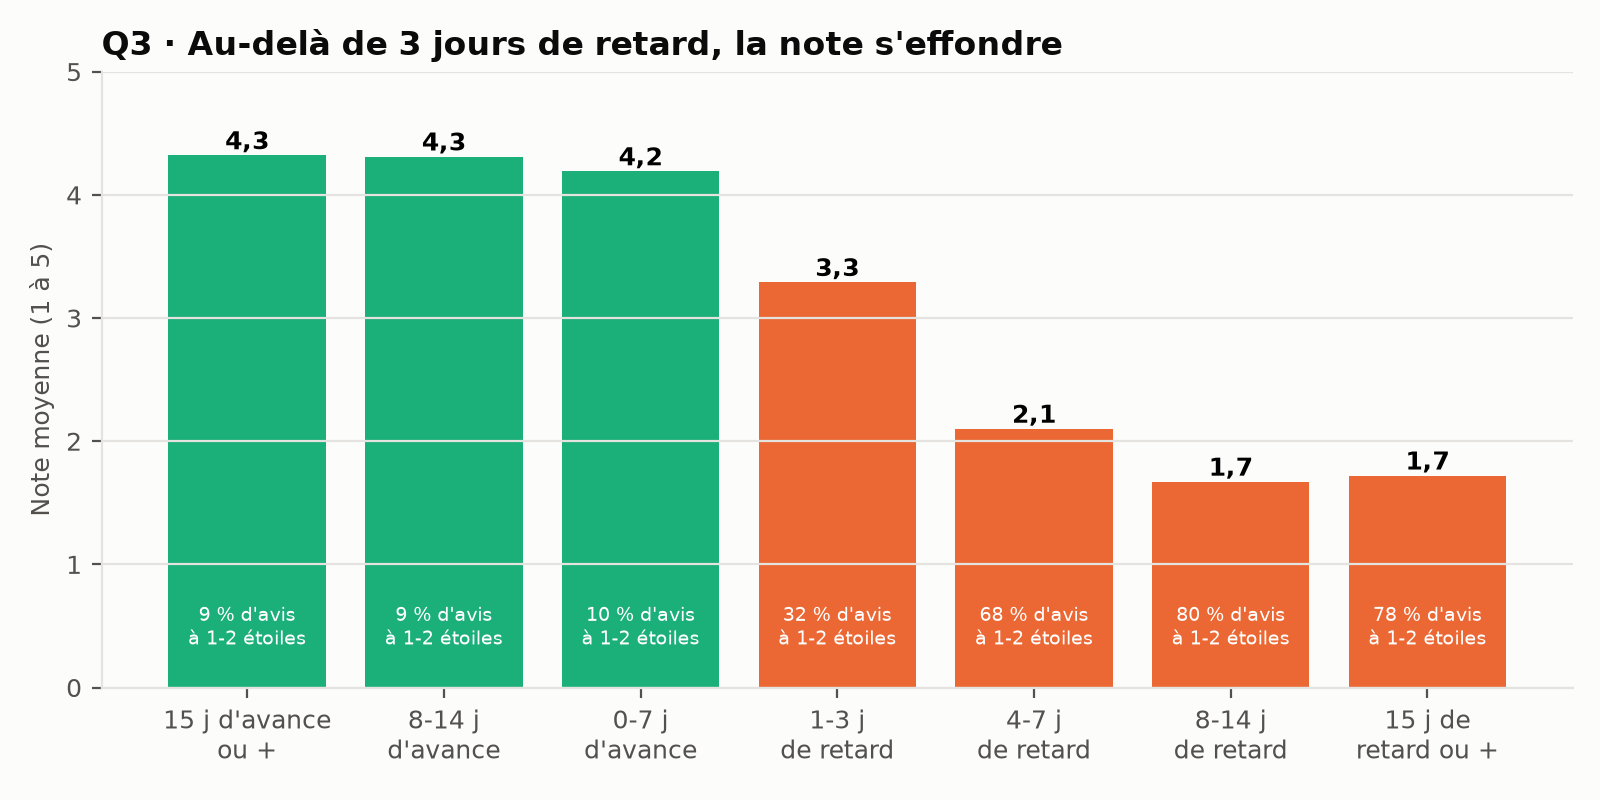
\includegraphics[width=0.86\linewidth]{q3_note_selon_retard.png}
\end{figure}
6,8~\% des commandes livrées arrivent en retard. La note moyenne tombe de \textbf{4,3} (à l'heure ou en avance) à \textbf{2,1} entre 4 et 7 jours
de retard. Au-delà d'une semaine, \textbf{80~\%} des avis sont à 1 ou 2 étoiles.

\subsection*{Q4 · Comment les clients paient-ils ?}
\begin{figure}[H]
\centering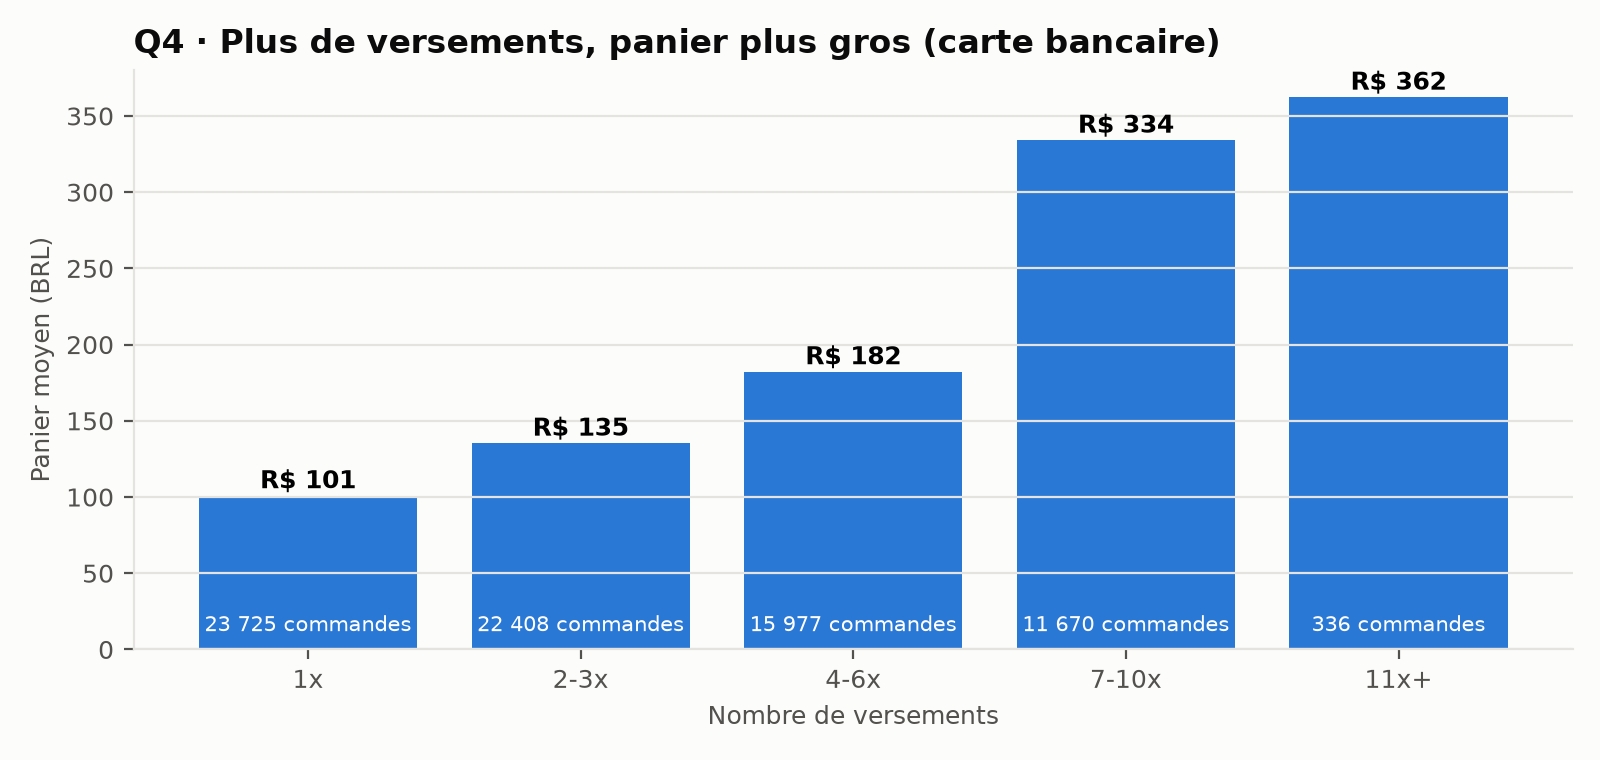
\includegraphics[width=0.86\linewidth]{q4_paiement_versements.png}
\end{figure}
La carte bancaire règle 75,5~\% des commandes, le \emph{boleto} (bordereau payé en espèces ou en ligne) 19,9~\%. Avec la carte, le panier
moyen passe de \textbf{101~BRL} en un versement à \textbf{334~BRL} en 7 à 10 versements.

\subsection*{Q5 · Combien pèse le fret ?}
\begin{figure}[H]
\centering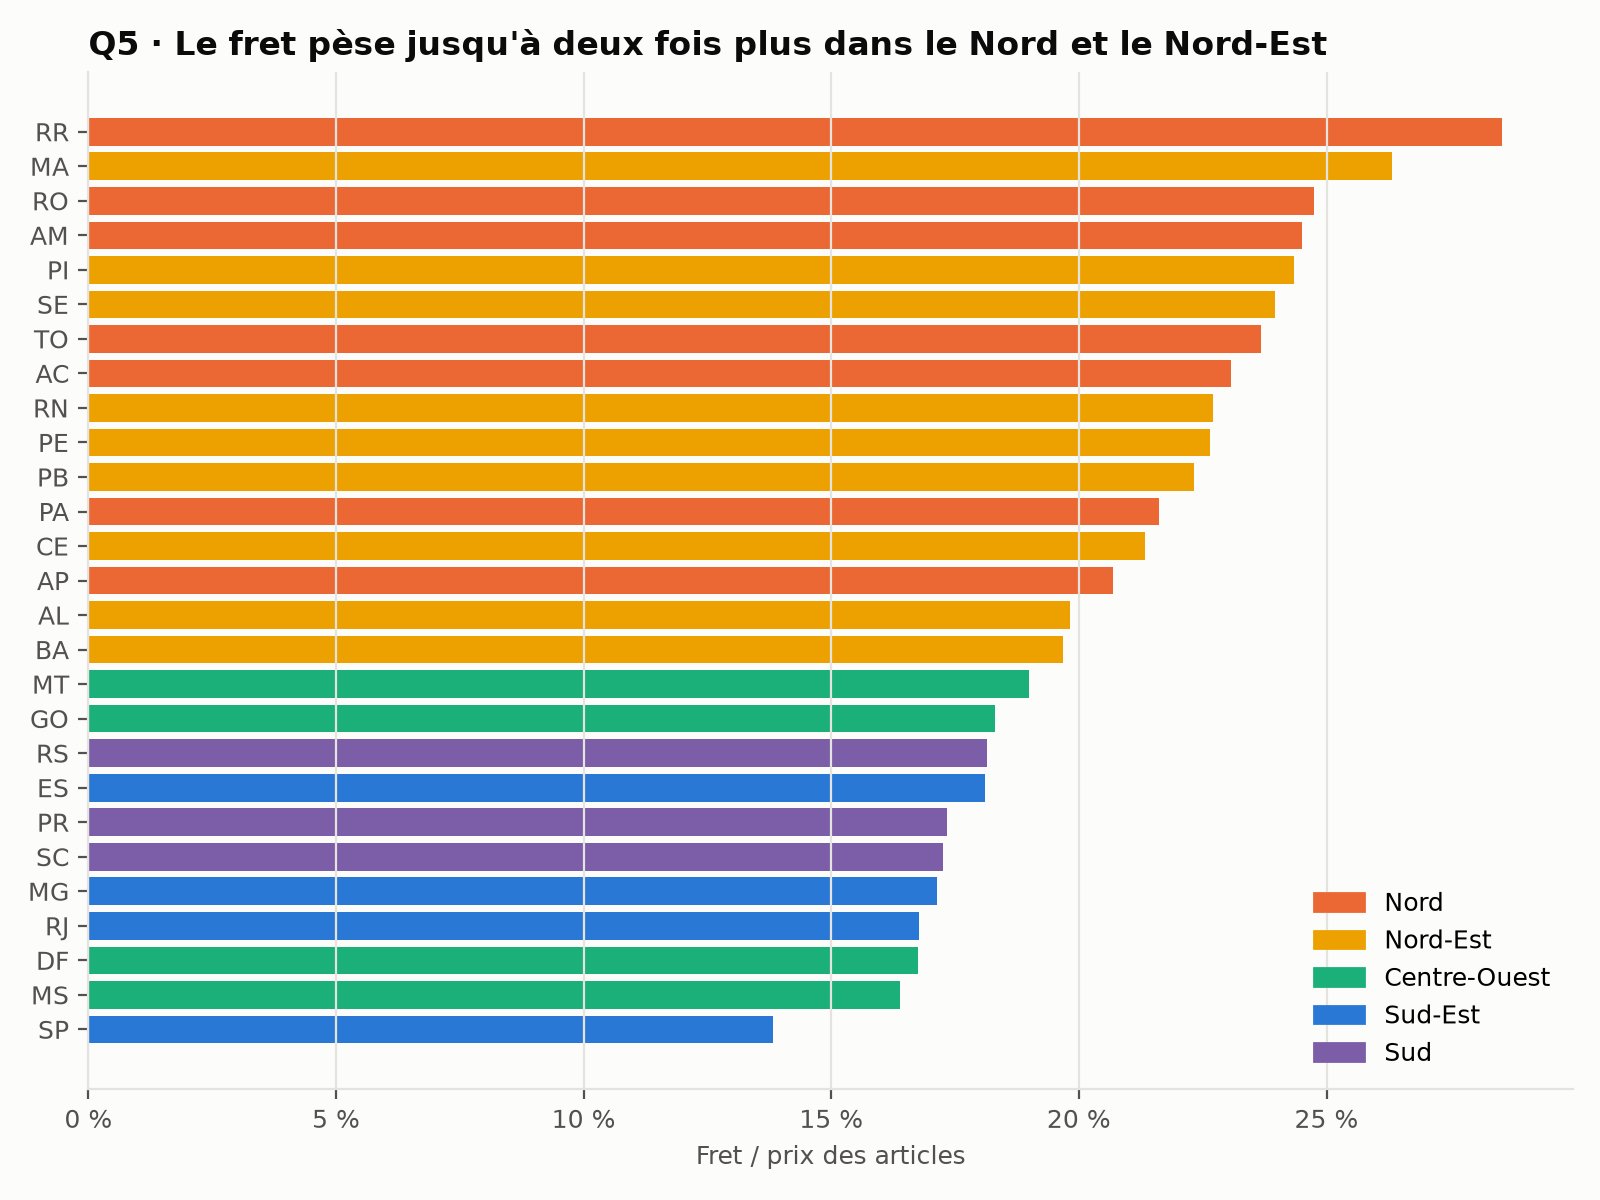
\includegraphics[width=0.78\linewidth]{q5_fret_par_etat.png}
\end{figure}
Le fret représente 13,8~\% du prix des articles à São Paulo (8,7 jours de livraison en moyenne), mais \textbf{jusqu'à 28,5~\%} dans le
Roraima (29 jours). Le Nord et le Nord-Est cumulent fret élevé, délais longs et retards plus fréquents.

\begin{keybox}[Recommandations au comité de direction]
\begin{enumerate}[leftmargin=1.4em]
  \item \textbf{Lancer avec le linge de maison et la décoration}, déjà 3\textsuperscript{e} et 6\textsuperscript{e} catégories du marché.
  \item \textbf{Commencer par le Sud-Est} (São Paulo, Rio, Minas Gerais) : 63~\% du CA, le fret le plus faible et les délais les plus courts.
        Le Nord et le Nord-Est viendront ensuite, avec une politique de fret dédiée.
  \item \textbf{Investir dans l'acquisition plutôt que dans la fidélisation} : 97~\% des clients n'achètent qu'une fois. Préparer le Black Friday.
  \item \textbf{Choisir le transporteur sur sa ponctualité} et promettre des délais réalistes : un retard de quelques jours divise la note par deux.
  \item \textbf{Proposer le paiement en plusieurs fois et le \emph{boleto}} : le panier moyen triple avec les versements.
\end{enumerate}
\end{keybox}

% =============================================================================
\section{Limites}
\begin{itemize}[leftmargin=1.2em]
  \item Les données couvrent 2016-2018 : elles décrivent la \textbf{structure} du marché, pas son état actuel. Elles proviennent d'une seule marketplace.
  \item Le chiffre d'affaires est celui de tous les vendeurs de la marketplace, pas celui d'une marque comparable à Maison Caju.
  \item L'entrepôt est reconstruit à chaque livraison (environ 20~s) : adapté à ce volume, pas à des centaines de millions de lignes.
  \item \texttt{dagster dev} regroupe serveur et démon dans un conteneur, avec un historique en SQLite : adapté à un poste, pas à la production.
\end{itemize}

% =============================================================================
\section{Retour d'expérience}
\begin{table}[H]
\centering\small
\begin{tabularx}{\linewidth}{@{}L{3.9cm} Y@{}}
\toprule
\textbf{Incident} & \textbf{Leçon} \\
\midrule
L'image MinIO n'est plus publiée & Un composant open source peut changer de modèle de distribution. Grâce au standard S3, SeaweedFS l'a remplacé \textbf{sans changer une ligne de code} (ADR 002) \\
dbt lancé avant la première commande & L'ordre de démarrage d'une plateforme est une dépendance comme une autre : il doit être \textbf{explicite} (amorçage, ADR 006) \\
\texttt{dagster-dbt} exige Python < 3.14 & Vérifier la compatibilité de \textbf{toute} la chaîne avant de choisir une version \\
Smart App Control bloque des DLL non signées ; une exécution figée 83 min bloque la file & Une file à exécution unique a besoin d'un \textbf{délai maximal}. La conteneurisation rend la plateforme indépendante du poste (ADR 005) \\
Le test du tableau de bord échoue dans la CI & La période par défaut était écrite en dur : un test sur d'autres données révèle les \textbf{hypothèses cachées} \\
Simulation des livraisons en 3 min 30 & Filtrer 26 fois une table coûte plus qu'un seul regroupement : 26~s après correction \\
\bottomrule
\end{tabularx}
\caption{Ce que ce projet a appris}
\end{table}

% =============================================================================
\section{Feuille de route}
\begin{enumerate}[leftmargin=1.4em]
  \item \textbf{Passage au cloud} (projet 6) : lac sur Google Cloud Storage, entrepôt BigQuery, même structure dbt, infrastructure en code.
  \item \textbf{Modèles dbt incrémentaux} si le volume ou la fréquence augmentent.
  \item \textbf{Dagster en production} : serveur, démon et base PostgreSQL séparés ; alertes en cas d'échec.
  \item \textbf{Fraîcheur des sources} : alerte si aucune livraison n'arrive en 35 jours (\texttt{dbt source freshness}, déjà configuré).
  \item \textbf{Analyse des avis} (texte en portugais) pour comprendre les causes d'insatisfaction.
\end{enumerate}

% =============================================================================
\clearpage
\appendix
\section{Arborescence du dépôt}
\begin{lstlisting}[language={}]
src/olist_pipeline/   config, landing, bronze, definitions (Dagster), dbt_cli, report
dbt/models/           staging (9) · intermediate (2) · marts/core (6) · marts/reporting (5)
dbt/tests/            3 rapprochements avec la source
dashboard/app.py      tableau de bord Streamlit (FR/EN)
tests/                pytest + échantillon CI (450 commandes réelles)
dagster_home/         configuration Dagster (concurrence, surveillance)
docs/                 mission, ADR, journal, dictionnaire, rapports, recette
Dockerfile · docker-compose.yml · .github/workflows/ci.yml
\end{lstlisting}

\section{Étapes de l'intégration continue}
\begin{enumerate}[leftmargin=1.4em]
  \item Style du code (\texttt{ruff}) et tests Python (\texttt{pytest}).
  \item Livraisons simulées à partir de l'échantillon, puis ingestion dans un lac local (dossier).
  \item \texttt{dbt build} : 22 modèles, 69 tests de données, 3 tests unitaires.
  \item Validation des définitions Dagster, test de fumée du tableau de bord.
  \item Construction de l'image Docker.
\end{enumerate}

\end{document}
